\section{Langkah-Langkah Percobaan}
%%%%%%%%%%%%%%%%%%%%%%%%%%%%%%%%%%%%%%%%%%%%%%%%%%
\subsection{Wireless Point to Point}
\begin{enumerate}
    \item Kabel LAN dihubungkan dari laptop ke router, dan router ke router.
    \item Login menggunakan MAC address, lalu router direset terlebih dahulu menggunakan Winbox.
    \begin{figure}[H]
        \centering
        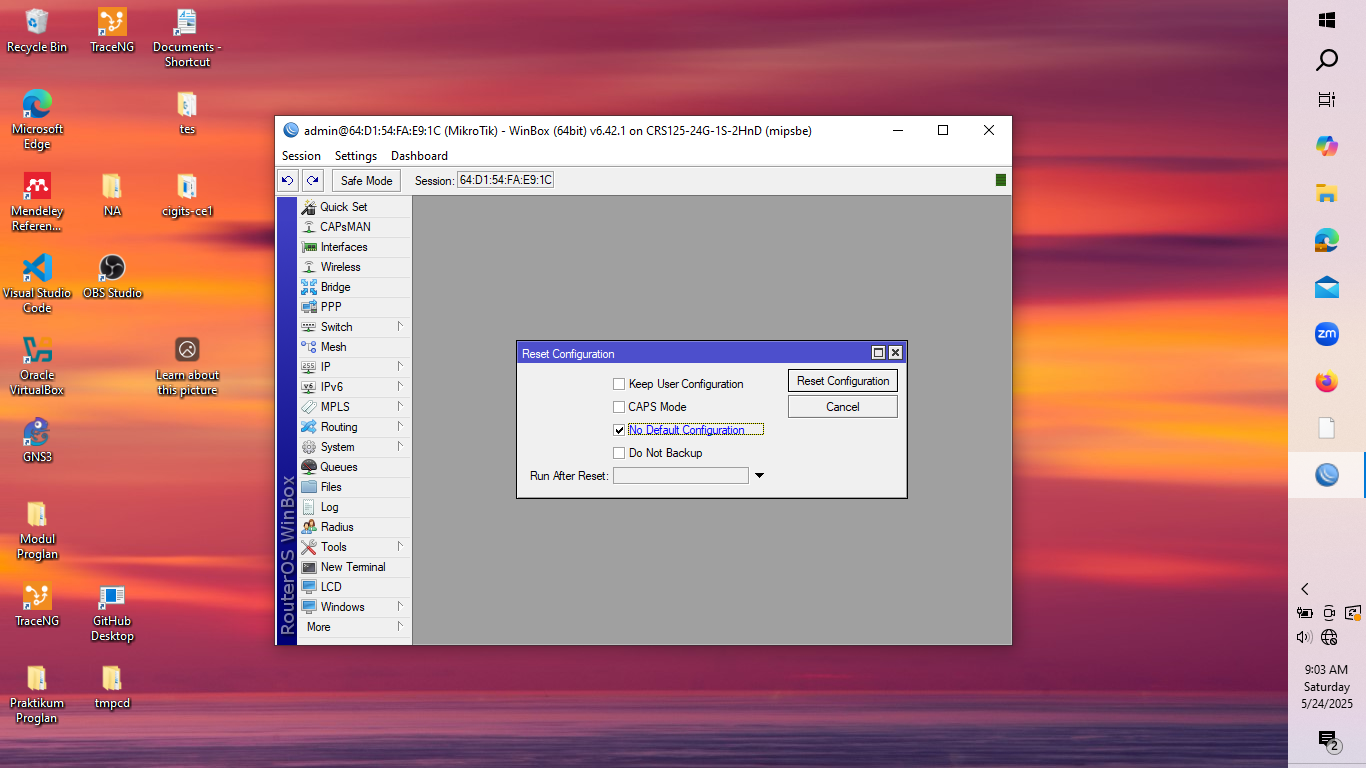
\includegraphics[width=0.5\linewidth]{gambar1.png}
        \caption{Mereset Router pada Winbox}
        \label{fig:reset-router}
    \end{figure}

    \item Aktifkan interface wireless wlan1. Masuk ke menu Wireless > WiFi Interfaces, klik interface wlan1, dan tekan ikon panah biru untuk mengaktifkannya. Ganti mode menjadi \textbf{bridge} dengan SSID \texttt{PointToPoint\_16}.

    \item Untuk Router B, aktifkan interface wlan1 dan ubah mode menjadi \textbf{station}.
    \begin{figure}[H]
        \centering
        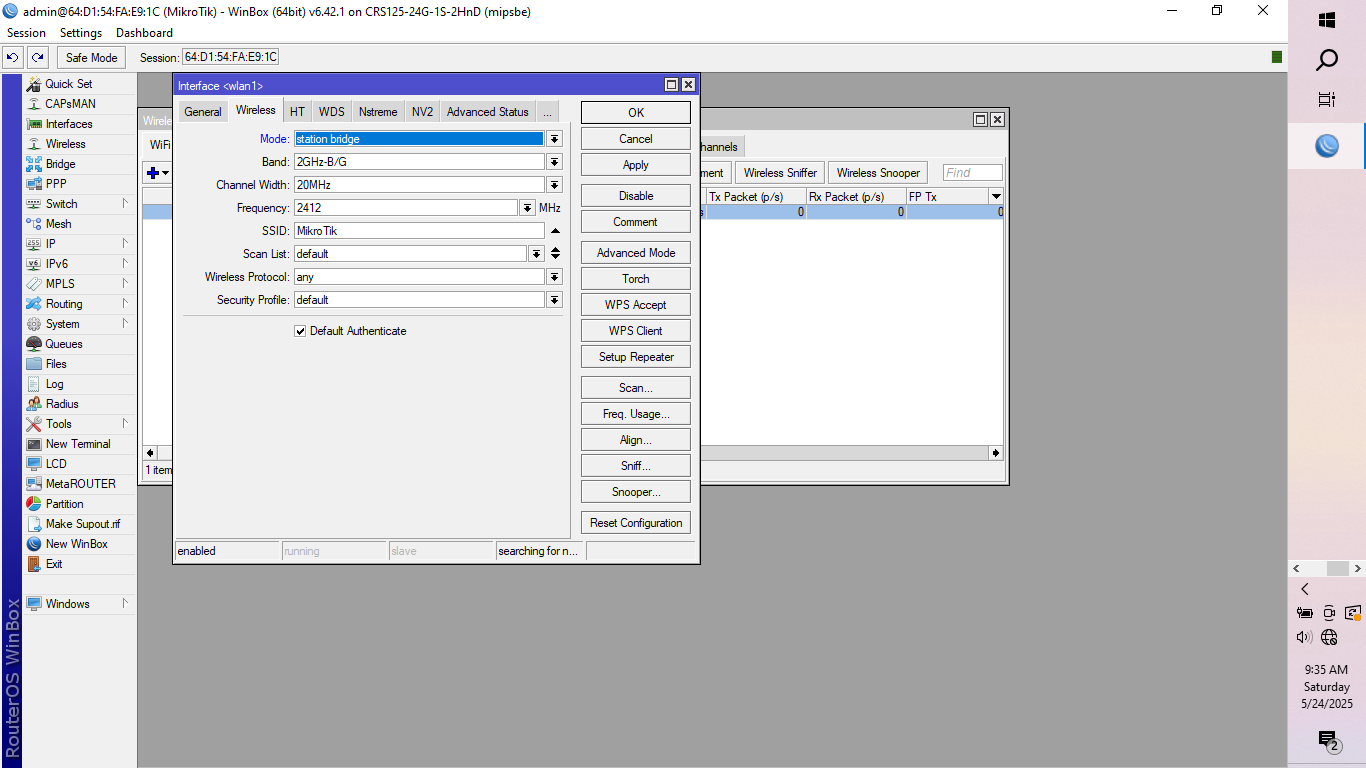
\includegraphics[width=0.5\linewidth]{gambar3a.png}
        \caption{Mengaktifkan Interface Wireless pada Router B}
        \label{fig:aktif-wlan-b}
    \end{figure}

    \item Pada Laptop B, klik tombol Scan, pilih SSID \texttt{PointToPoint\_16}, lalu klik \textit{Connect}.
    \begin{figure}[H]
        \centering
        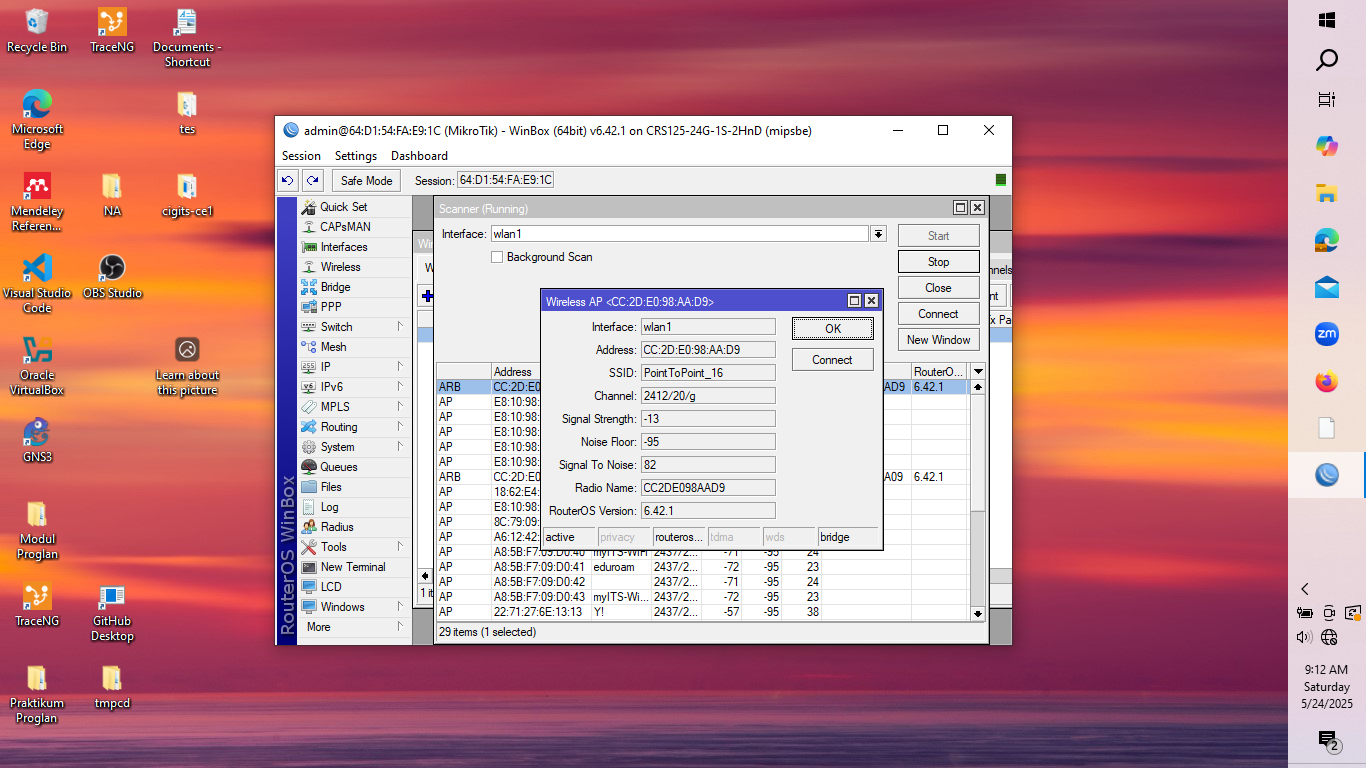
\includegraphics[width=0.5\linewidth]{gambar3.png}
        \caption{Menghubungkan Laptop B ke Router A}
        \label{fig:hubungkan-laptop}
        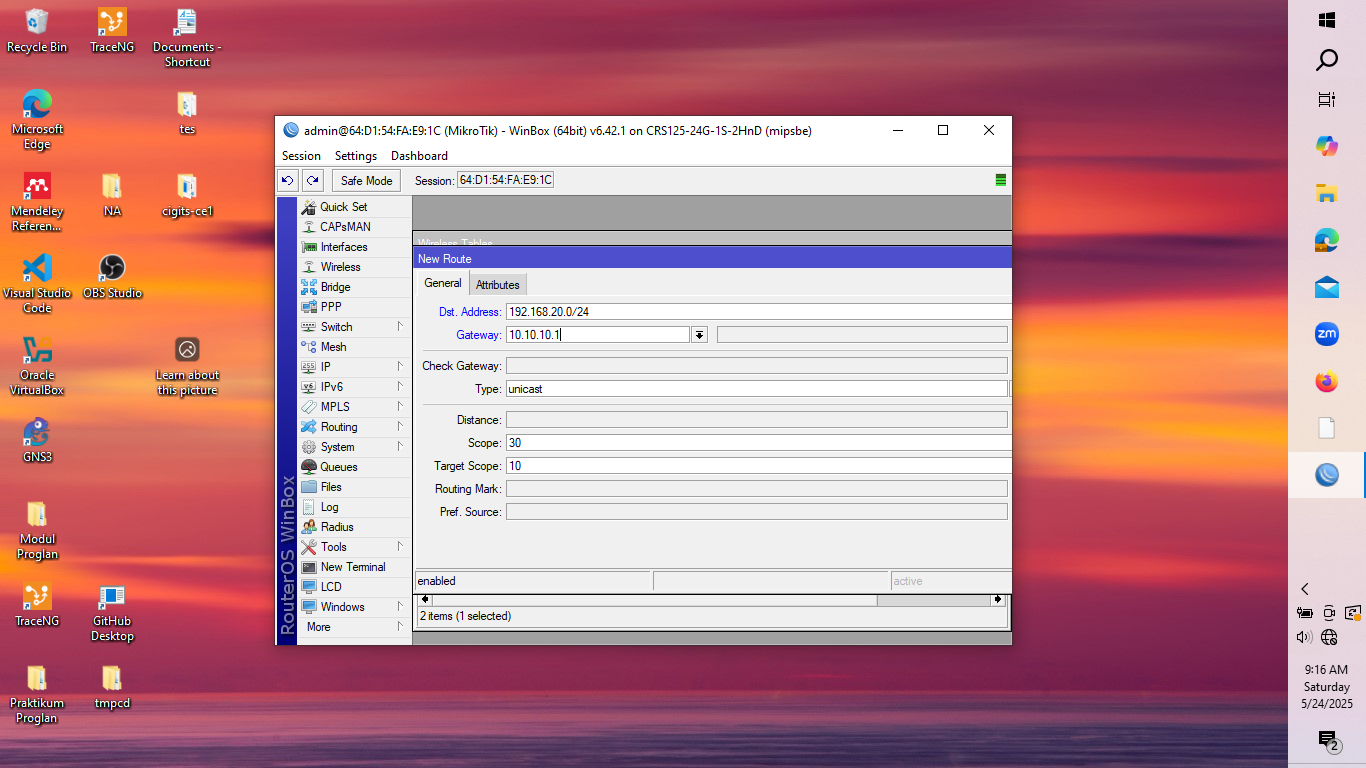
\includegraphics[width=0.5\linewidth]{gambar5.png}
        \caption{Konfigurasi IP Address Laptop}
        \label{fig:ip-laptop}
    \end{figure}

    \item Lakukan pengujian koneksi dengan ping dari Laptop A ke B dan sebaliknya.
    \begin{figure}[H]
        \centering
        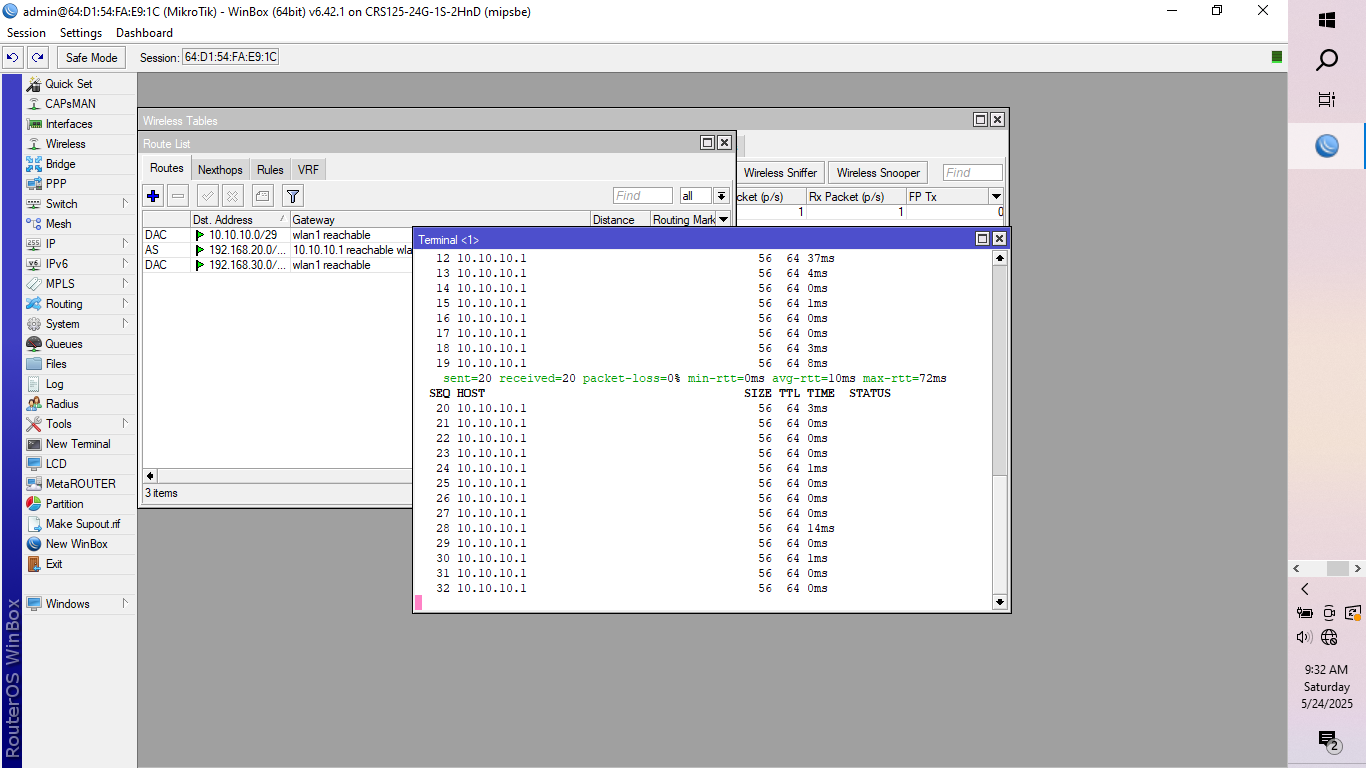
\includegraphics[width=0.5\linewidth]{ping1.png}
        \caption{Ping dari Laptop A ke Laptop B}
        \label{fig:ping-ptp}
    \end{figure}
\end{enumerate}

%%%%%%%%%%%%%%%%%%%%%%%%%%%%%%%%%%%%%%%%%%%%%%%%%%%%%%%%%%%%%%%%%%%%%%%%%%%%%%%%%%%%

\subsection{Wireless Point to Multipoint}
\begin{enumerate}
    \item Kabel LAN dihubungkan dari laptop ke router, dan router ke router.
    \item Login menggunakan MAC address, lalu router direset terlebih dahulu menggunakan Winbox.
    \begin{figure}[H]
        \centering
        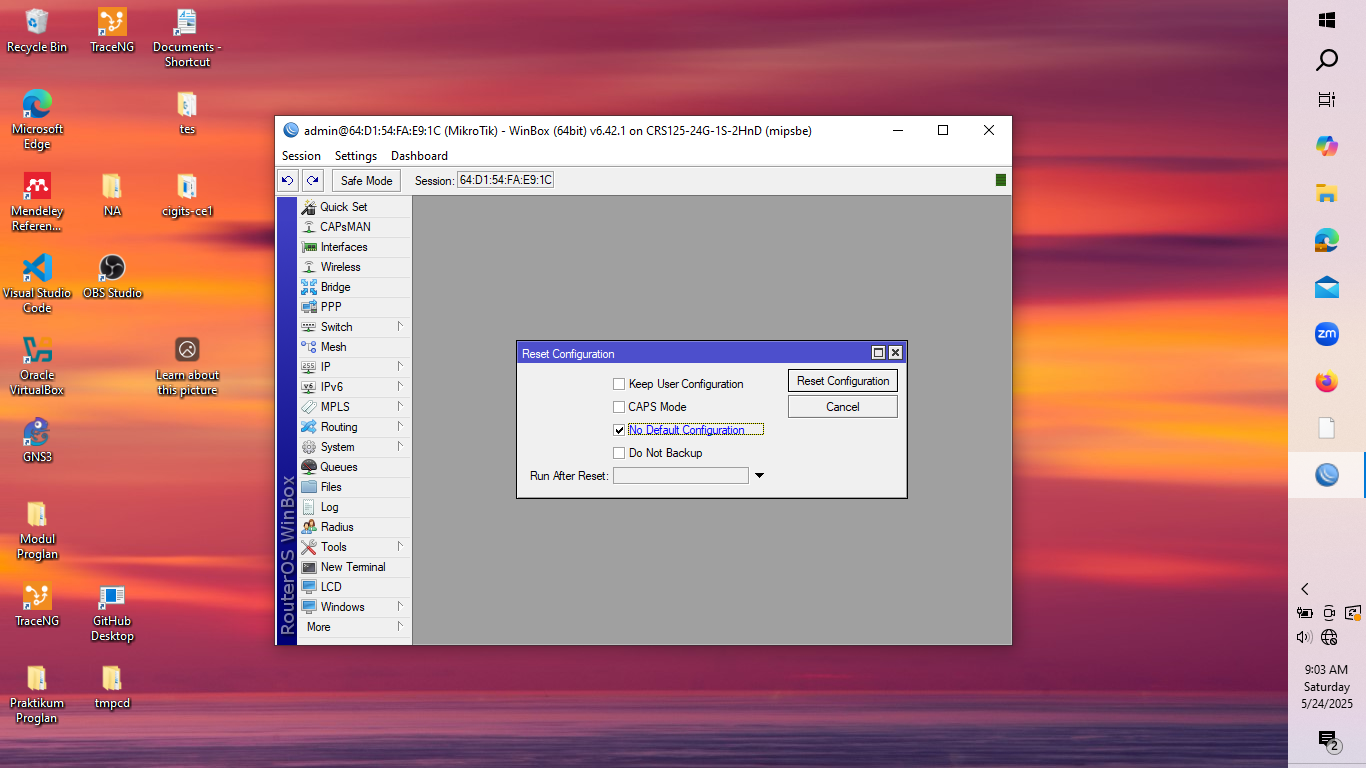
\includegraphics[width=0.5\linewidth]{gambar1.png}
        \caption{Mereset Router pada Winbox}
        \label{fig:reset-router-multi}
    \end{figure}

    \item Aktifkan wlan1 pada Router A, ubah mode menjadi \textbf{AP bridge} dengan SSID \texttt{PointToMultiPoint\_16}.
 

    \item Pada Router B, aktifkan wlan1 dan ubah mode menjadi \textbf{station bridge}.
    \begin{figure}[H]
        \centering
        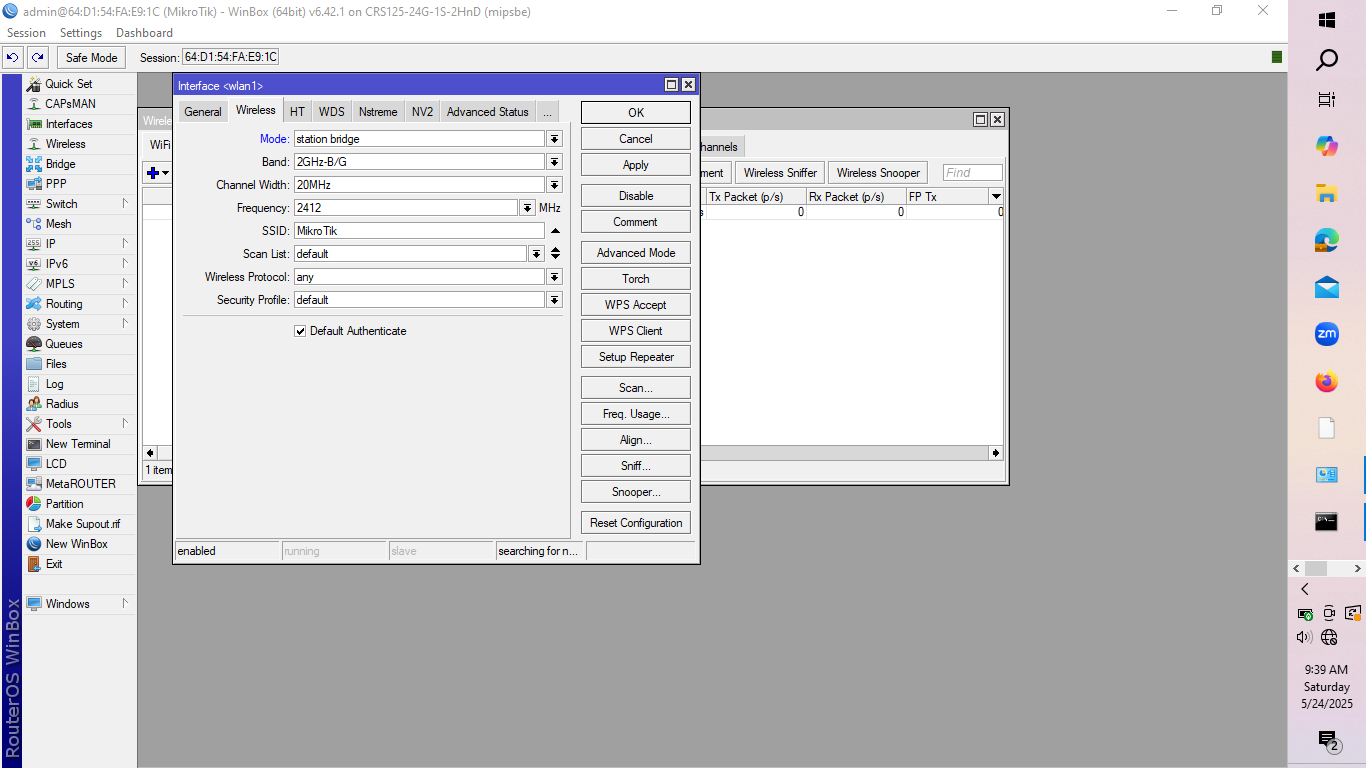
\includegraphics[width=0.5\linewidth]{gambar3ma.png}
        \caption{Mengaktifkan Interface Wireless pada Router B (Multipoint)}
        \label{fig:aktif-wlan-b-multi}
    \end{figure}

    \item Pada Laptop B, klik tombol Scan, pilih SSID \texttt{PointToMultiPoint\_16}, lalu klik Connect.
    \begin{figure}[H]
        \centering
        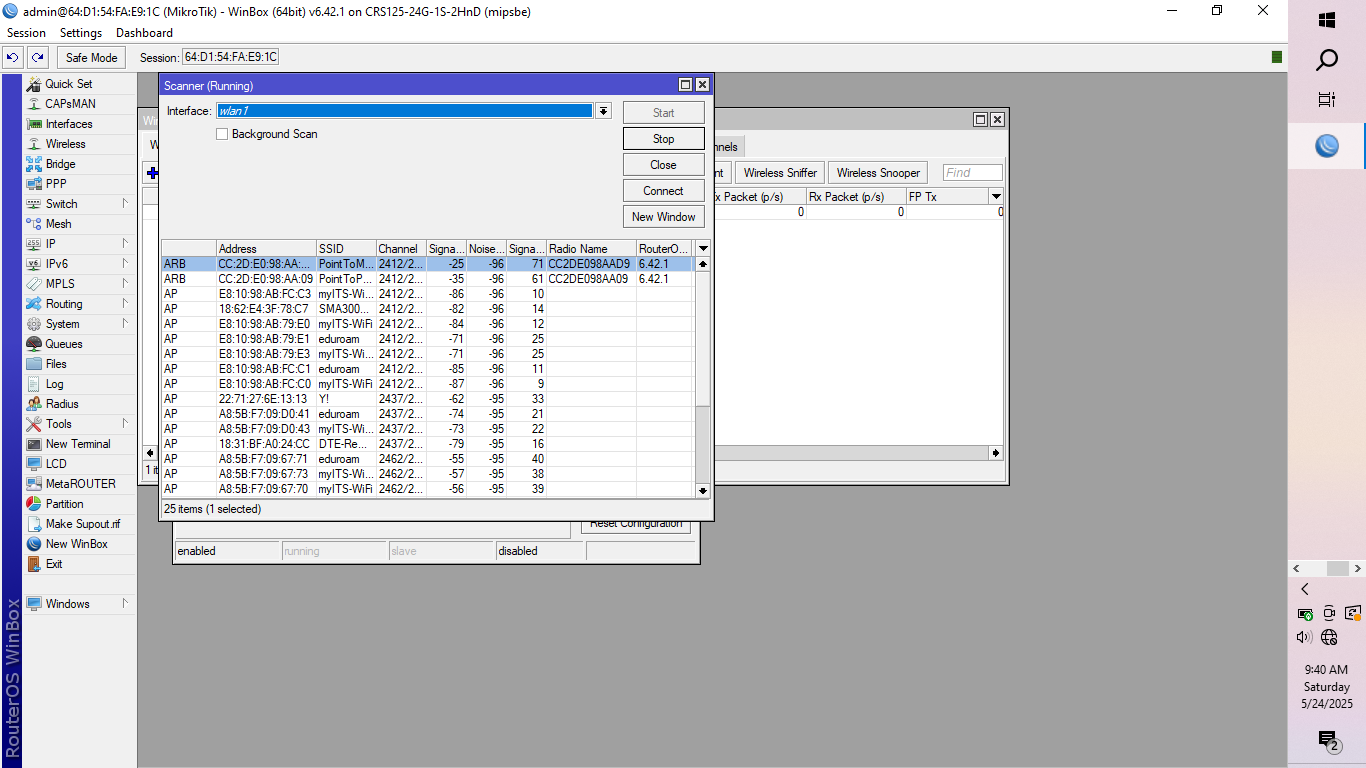
\includegraphics[width=0.5\linewidth]{gambar3m.png}
        \caption{Menghubungkan Laptop B ke Router A (Multipoint)}
        \label{fig:hubungkan-laptop-multi}
    \end{figure}

    \item Konfigurasikan IP WLAN dan ether2 pada kedua router.
    \begin{figure}[H]
        \centering
        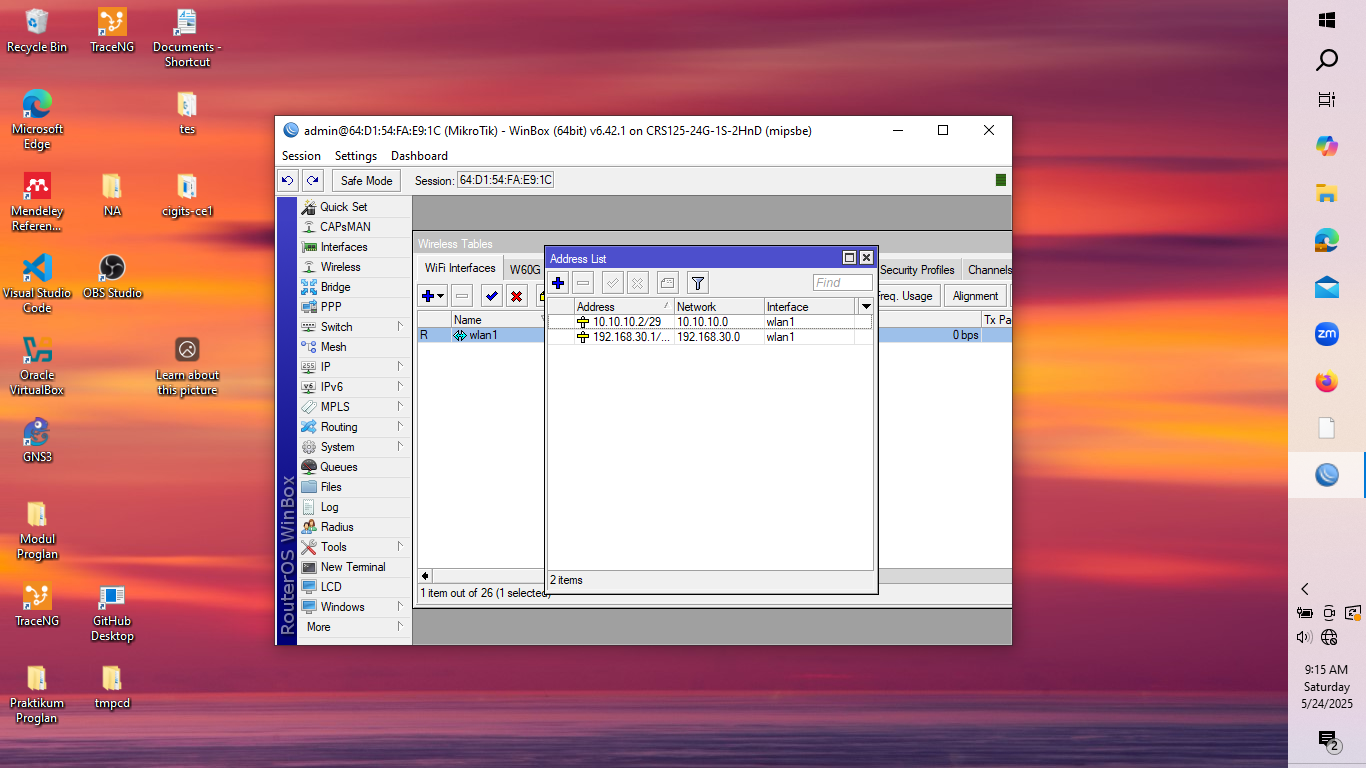
\includegraphics[width=0.5\linewidth]{gambar4.png}
        \caption{Mengkonfigurasi IP Address pada Router A dan B (Multipoint)}
        \label{fig:ip-router-multi}
    \end{figure}

    \item Tambahkan routing statis.
    \begin{figure}[H]
        \centering
        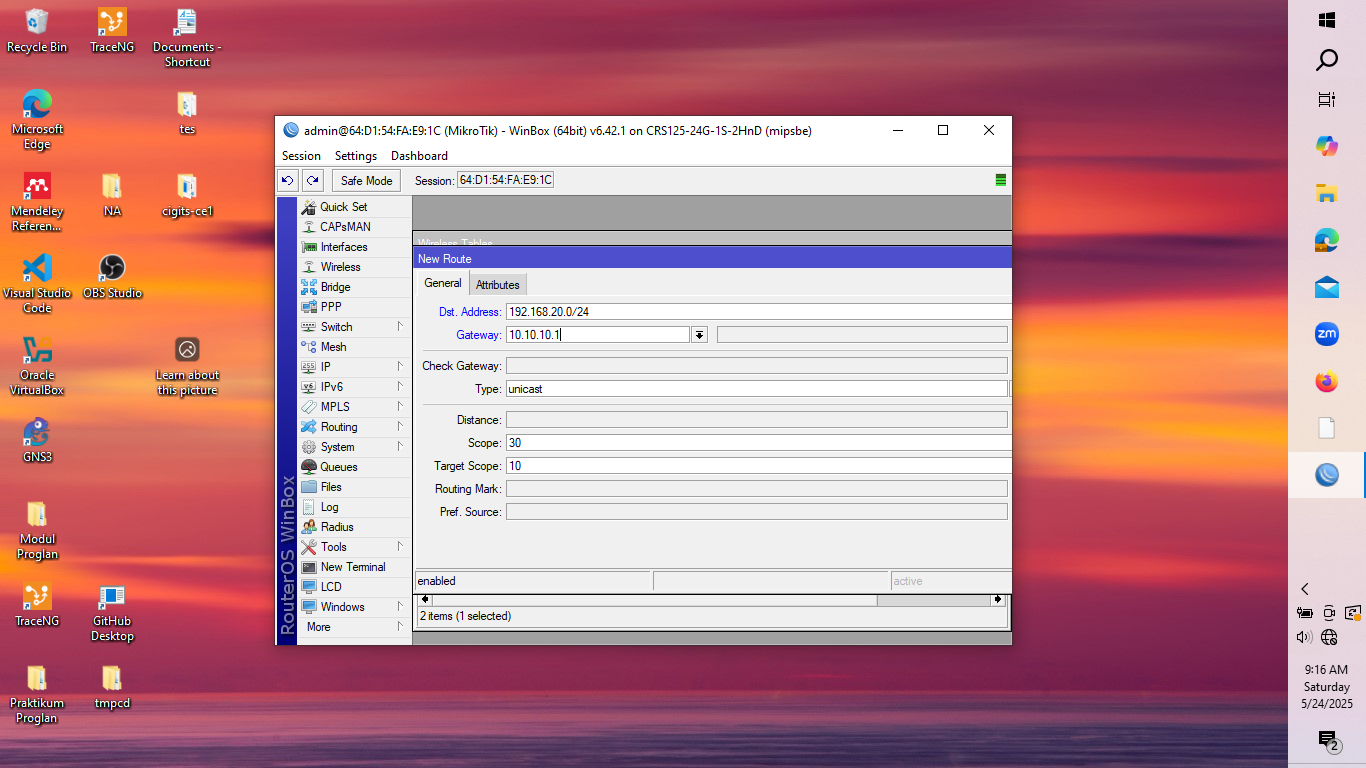
\includegraphics[width=0.5\linewidth]{gambar5.png}
        \caption{Menambahkan Routing Statis pada Router A dan B (Multipoint)}
        \label{fig:routing-multi}
    \end{figure}

    \item Konfigurasikan IP address laptop melalui Control Panel.
    \begin{figure}[H]
        \centering
        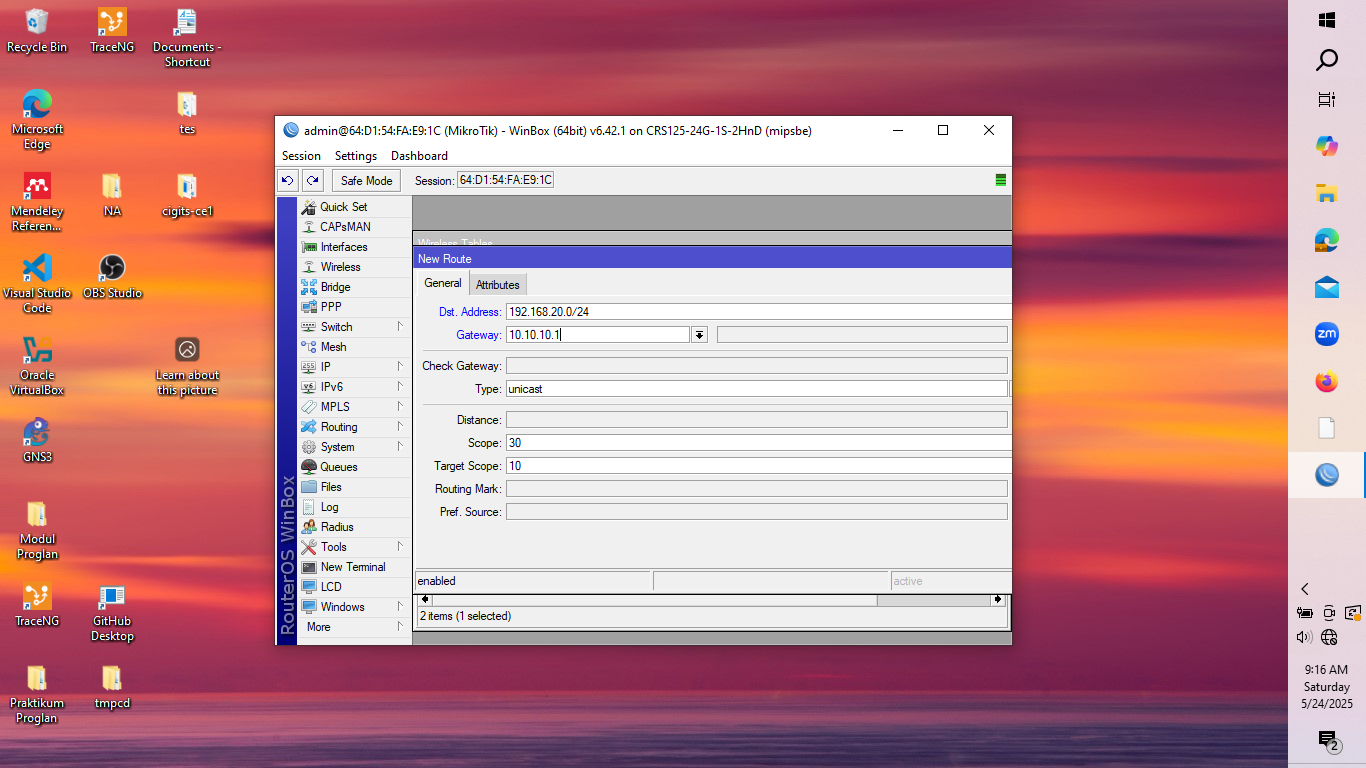
\includegraphics[width=0.5\linewidth]{gambar5.png}
        \caption{Konfigurasi IP Address Laptop (Multipoint)}
        \label{fig:ip-laptop-multi}
    \end{figure}

    \item Uji koneksi dengan ping dari Laptop A ke Laptop B.
    \begin{figure}[H]
        \centering
        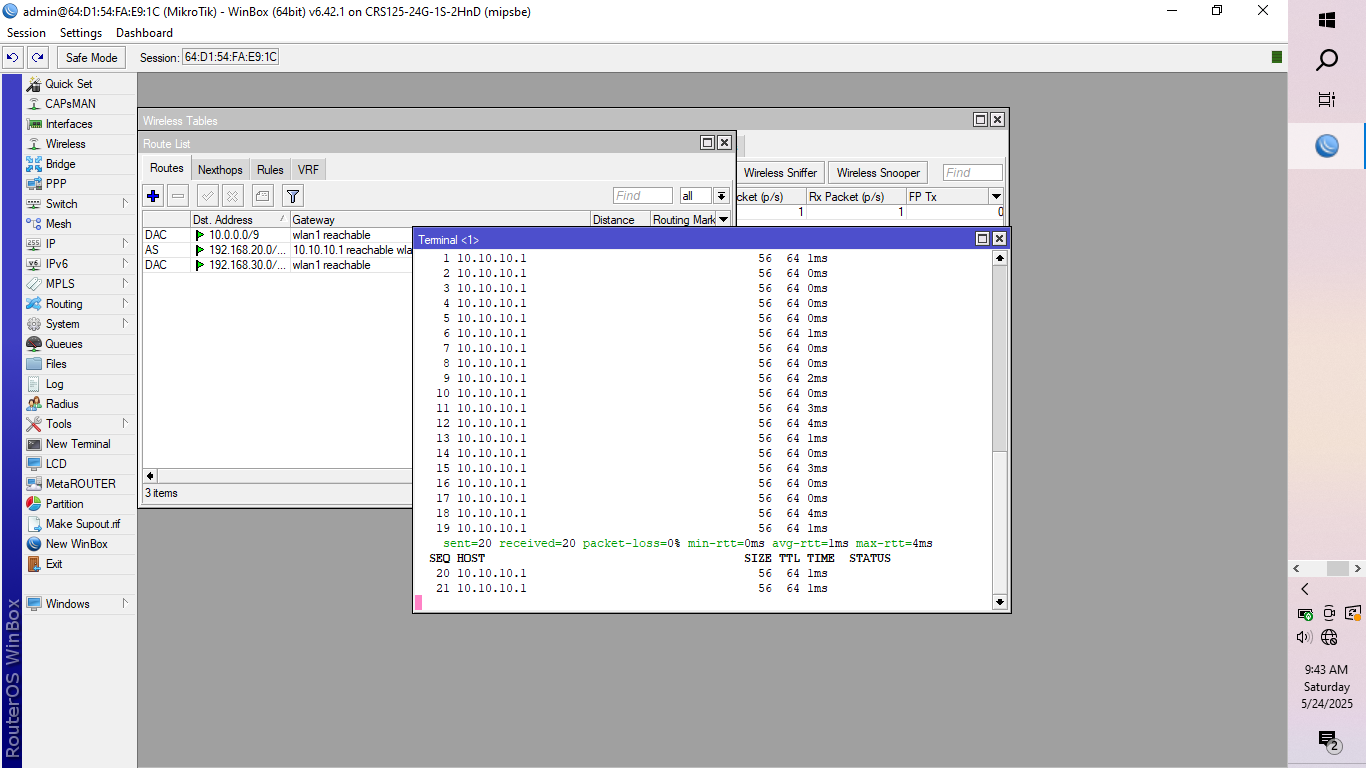
\includegraphics[width=0.5\linewidth]{ping2.png}
        \caption{Ping dari Laptop A ke Laptop B (Multipoint)}
        \label{fig:ping-multi}
    \end{figure}
\end{enumerate}

%%%%%%%%%%%%%%%%%%%%%%%%%%%%%%%%%%%%%%%%%%%%%%%%%%%%%%%%%%%%%%%%%%%%%%%%%%%%%%%%%%
\subsection{Wireless Bridge}
\begin{enumerate}
    \item Kabel LAN dihubungkan dari laptop ke router, dan router ke router.
    \item Login menggunakan MAC address, lalu reset router menggunakan Winbox.
    \begin{figure}[H]
        \centering
        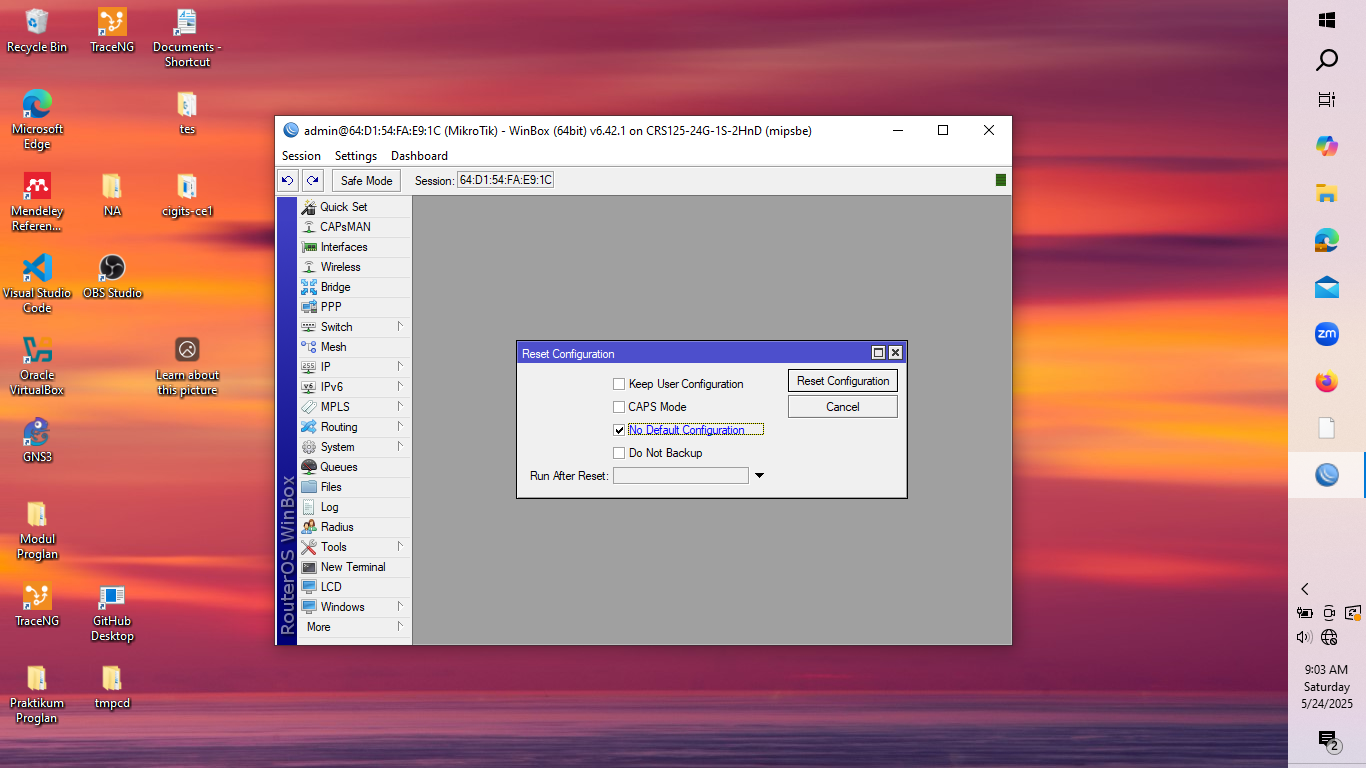
\includegraphics[width=0.5\linewidth]{gambar1.png}
        \caption{Mereset Router pada Winbox}
        \label{fig:reset-bridge}
    \end{figure}

    \item Aktifkan wlan1 pada Router A, ubah mode menjadi \textbf{bridge}, SSID \texttt{WirelessBridge\_16}.


    \item Aktifkan wlan1 Router B, ubah menjadi \textbf{station pseudobridge}.
    \begin{figure}[H]
        \centering
        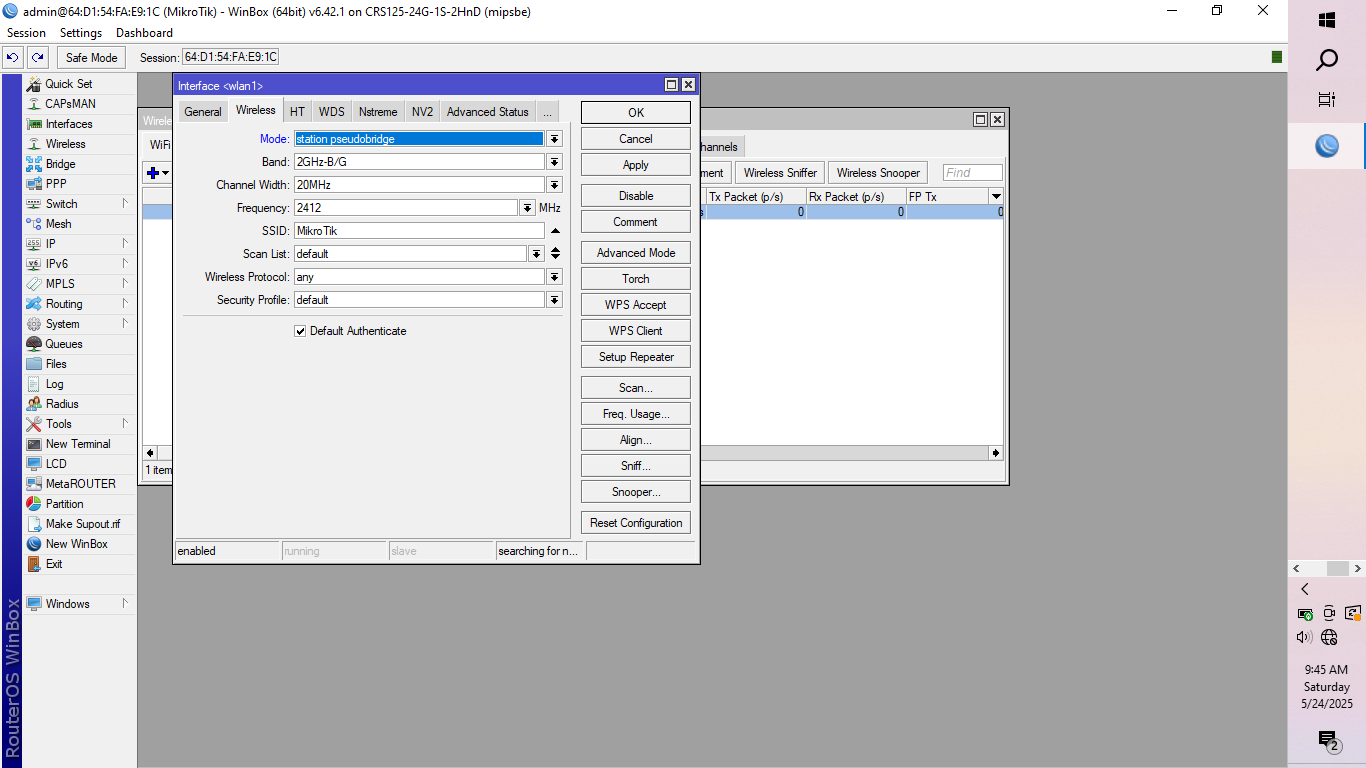
\includegraphics[width=0.5\linewidth]{gambar3w.png}
        \caption{Aktifkan Wireless Interface Router B (Bridge)}
        \label{fig:wlan-b-bridge}
    \end{figure}

    \item Scan dan hubungkan ke SSID \texttt{WirelessBridge\_16}.
    \begin{figure}[H]
        \centering
        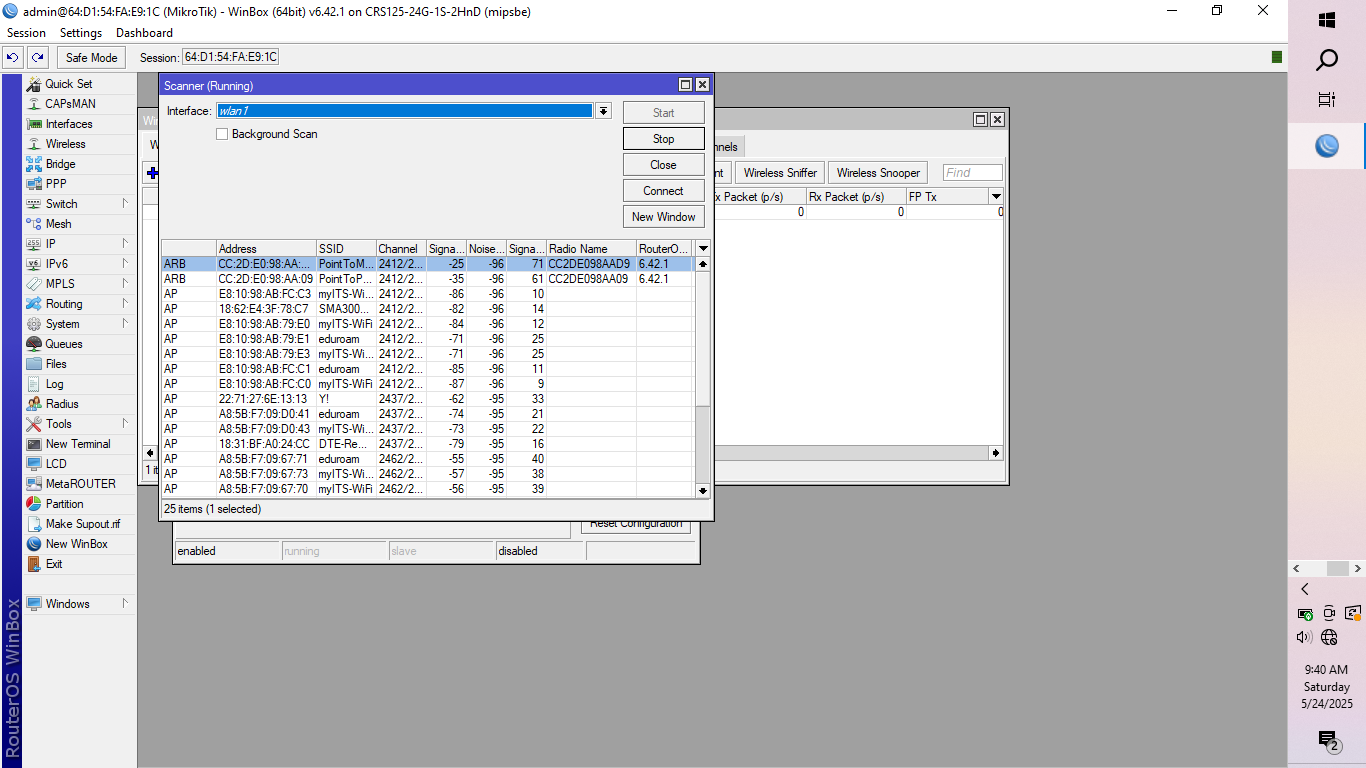
\includegraphics[width=0.5\linewidth]{gambar3m.png}
        \caption{Menghubungkan ke SSID Wireless Bridge}
        \label{fig:ssid-bridge}
    \end{figure}

    \item Konfigurasikan IP di wlan dan ether2.
    \begin{figure}[H]
        \centering
        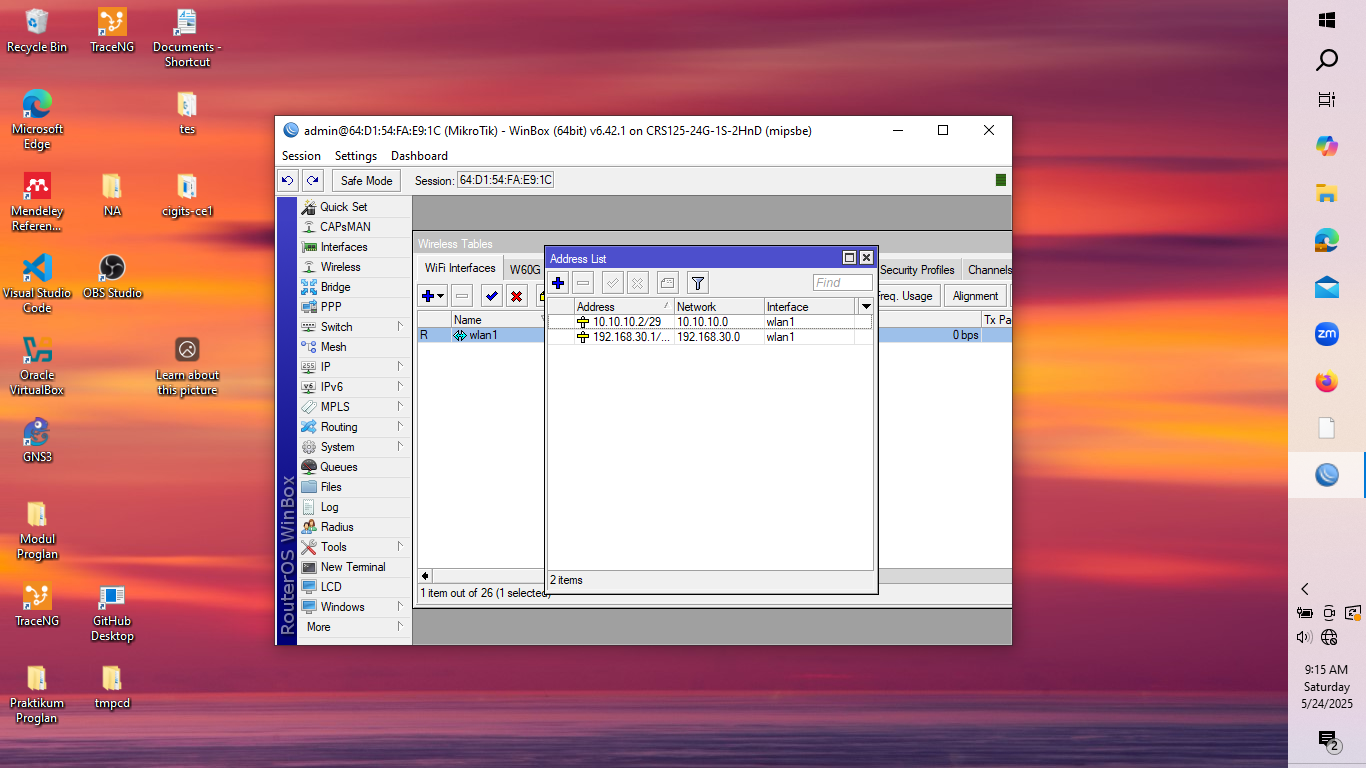
\includegraphics[width=0.5\linewidth]{gambar4.png}
        \caption{IP Configuration pada Router A dan B (Bridge)}
        \label{fig:ip-bridge}
    \end{figure}

    \item Tambahkan routing statis.
    \begin{figure}[H]
        \centering
        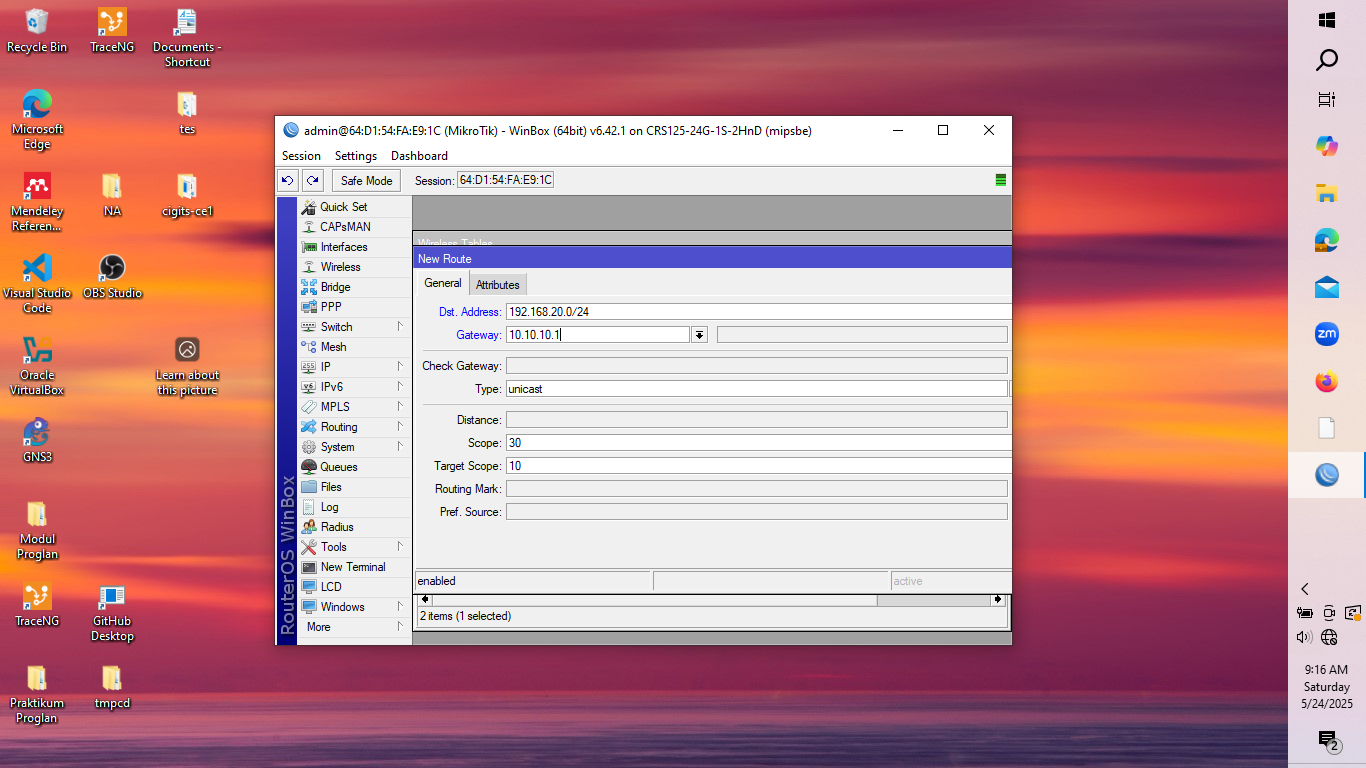
\includegraphics[width=0.5\linewidth]{gambar5.png}
        \caption{Routing Statis pada Router A dan B (Bridge)}
        \label{fig:routing-bridge}
    \end{figure}

    \item Konfigurasi IP laptop.
    \begin{figure}[H]
        \centering
        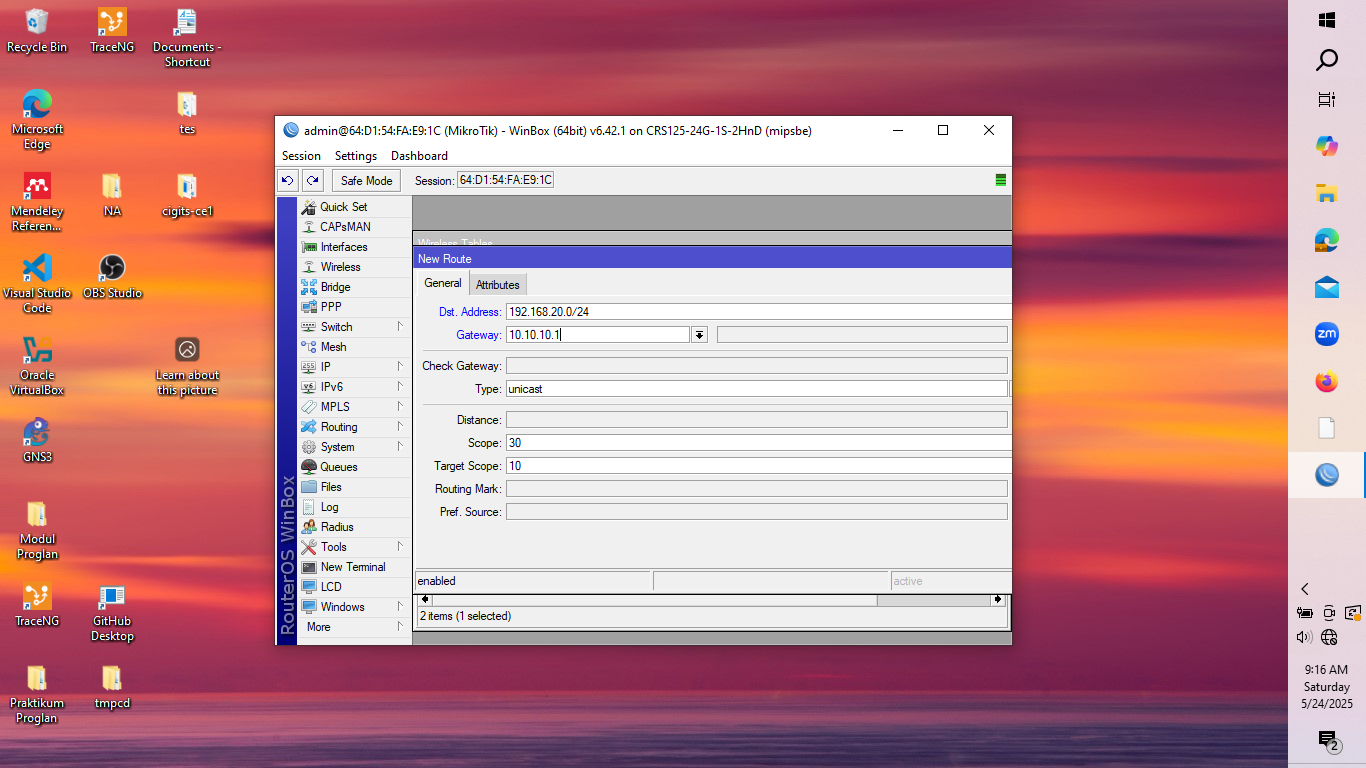
\includegraphics[width=0.5\linewidth]{gambar5.png}
        \caption{Konfigurasi IP Address Laptop (Bridge)}
        \label{fig:ip-laptop-bridge}
    \end{figure}
    
    \item Uji koneksi via ping.
    \begin{figure}[H]
        \centering
        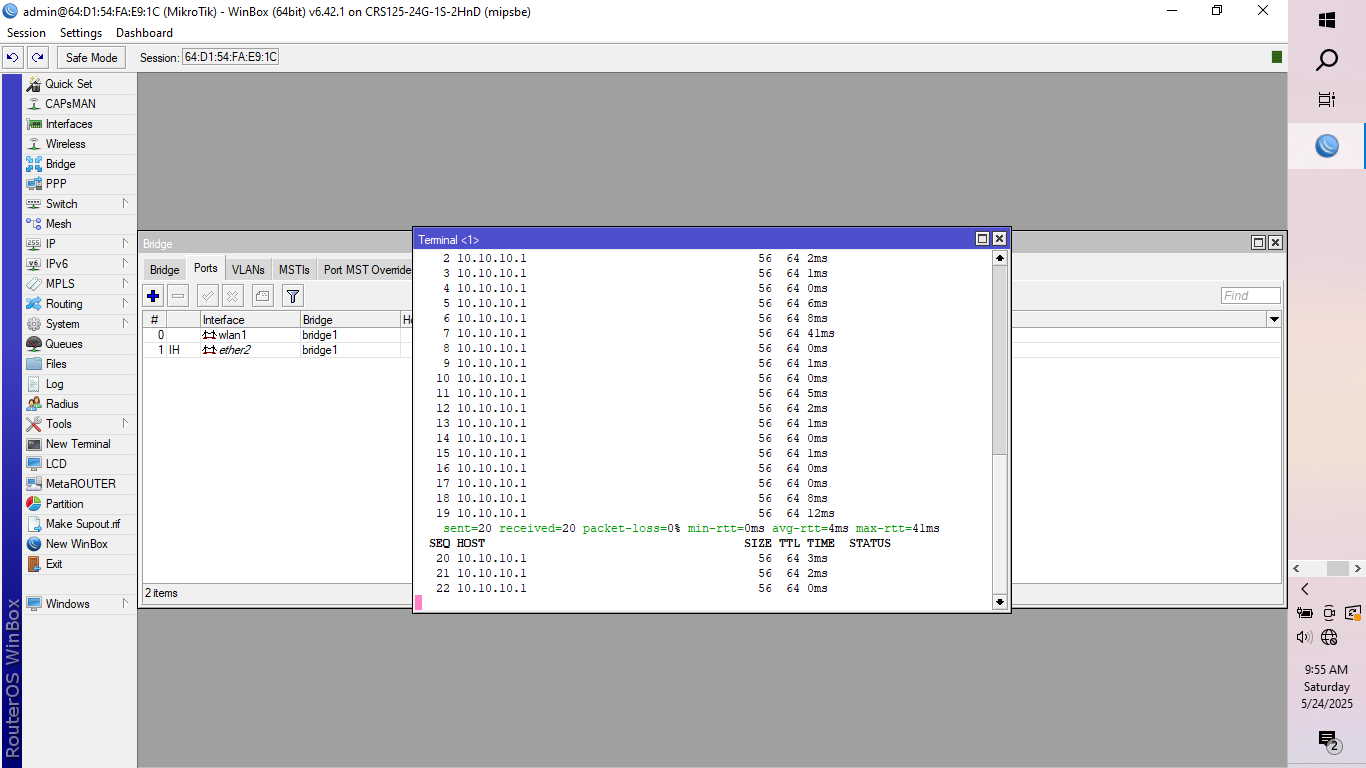
\includegraphics[width=0.5\linewidth]{ping3.png}
        \caption{Ping antara Laptop A dan B (Bridge)}
        \label{fig:ping-bridge}
    \end{figure}
\end{enumerate}



\section{Analisis Hasil Percobaan}
Pada percobaan ini dilakukan tiga jenis konfigurasi jaringan nirkabel menggunakan perangkat router, 
yaitu Wireless Point to Point, Wireless Point to Multipoint, dan Wireless Bridge. Masing-masing 
topologi memiliki tujuan dan karakteristik yang berbeda serta menunjukkan hasil yang bervariasi.

Pada konfigurasi Wireless Point to Point, dua router dikonfigurasikan agar dapat saling terhubung 
secara langsung. Router A diatur dalam mode bridge, sedangkan Router B sebagai station, dengan SSID 
yang sama yaitu PointToPoint16. Setelah IP address dan routing statis dikonfigurasikan, dilakukan 
uji koneksi menggunakan perintah ping dari Laptop A ke Laptop B. Hasil pengujian menunjukkan bahwa 
koneksi berjalan dengan baik, ditandai dengan waktu respon yang rendah dan tidak terjadi packet loss. 
Topologi ini cocok digunakan untuk menghubungkan dua titik secara langsung dengan koneksi yang stabil 
dan bandwidth yang optimal.

Pada konfigurasi Wireless Point to Multipoint, Router A diatur sebagai AP bridge yang berfungsi 
sebagai pusat koneksi, sementara Router B dikonfigurasikan sebagai station bridge untuk terhubung ke 
SSID PointToMultiPoint16. Topologi ini memungkinkan lebih dari satu client untuk terhubung ke satu 
access point. Setelah konfigurasi IP dan routing selesai, koneksi diuji melalui ping, dan hasilnya 
menunjukkan bahwa koneksi antar perangkat berhasil dilakukan.Topologi ini memerlukan 
pengelolaan jaringan yang lebih kompleks karena peningkatan jumlah client dapat menyebabkan penurunan 
performa jaringan akibat banyaknya sinyal dan berbagi bandwidth.

Sedangkan pada konfigurasi Wireless Bridge, tujuan utama adalah menyatukan dua jaringan lokal (LAN) 
melalui koneksi wireless. Router A kembali diatur sebagai bridge, namun Router B kali ini menggunakan 
mode station pseudobridge. Setelah koneksi wireless berhasil dan konfigurasi IP serta routing 
disesuaikan, uji koneksi melalui ping menunjukkan komunikasi dua arah berhasil dilakukan.Mode 
station pseudobridge memiliki keterbatasan dalam melewatkan semua jenis traffic, terutama yang 
bersifat broadcast atau multicast. Oleh karena itu, topologi ini lebih cocok untuk jaringan kecil 
atau skenario tertentu di mana bridging layer 2 dibutuhkan.



\section{Hasil Tugas Modul}

    \begin{figure}[H]
        \centering
        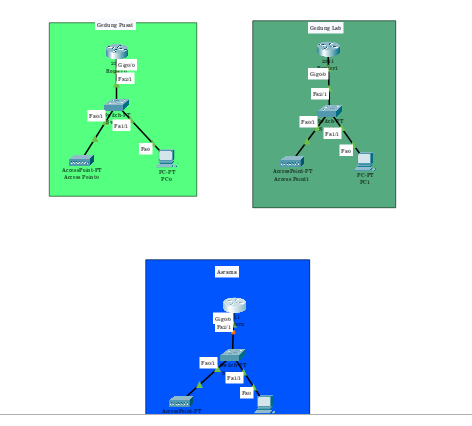
\includegraphics[width=0.5\linewidth]{topologi.png}
        \caption{Topologi jaringan}
        \label{fig:ping-bridge}
    \end{figure}
topologi ini menggambar
penghubungkan tiga gedung berbeda: Gedung Pusat, Gedung Lab, dan Gedung Asrama. Gedung Pusat 
berfungsi sebagai inti jaringan, di mana sebuah router utama mengelola alamat IP otomatis (DHCP) 
untuk perangkat lokal dan juga menjadi titik awal koneksi nirkabel ke gedung lainnya yang
menggunakan Access Point (AP) lokal di Gedung Pusat untuk menyediakan Wi-Fi bagi penggunanya. 
Untuk menghubungkan Gedung Lab dan Gedung Asrama Blok A ke Gedung Pusat, digunakan AP  
Point-to-Point (P2P) yang terhubung langsung ke router utama. AP ini bertindak sebagai pemancar 
sinyal nirkabel jarak jauh, memungkinkan router di Gedung Lab dan Gedung Asrama Blok A untuk 
terhubung sebagai penerima sinyal.

Di Gedung Lab dan Gedung Asrama Blok A, router lokal mereka bertindak sebagai pusat untuk jaringan 
masing-masing. Router ini menerima koneksi wirelessl dari Gedung Pusat melalui AP P2P
. Setelah menerima koneksi, router ini kemudian menyediakan jaringan lokal dengan 
alokasi IP otomatis (DHCP) dan Wi-Fi melalui AP lokal masing-masing. Perangkat di Blok B dapat langsung berkomunikasi dan 
mendapatkan IP dari server DHCP di Blok A, seolah-olah mereka berada dalam satu jaringan kabel yang 
sama, tanpa perlu routing tambahan di antara keduanya.


\section{Kesimpulan}
Berdasarkan hasil percobaan, dapat disimpulkan bahwa setiap konfigurasi jaringan nirkabel memiliki 
karakteristik dan keunggulan masing-masing. Konfigurasi Point to Point yang paling stabil 
dan efisien untuk komunikasi dua perangkat secara langsung. Konfigurasi Point to Multipoint 
memberikan fleksibilitas dalam jumlah client yang dapat terhubung, namun perlu mempertimbangkan 
manajemen bandwidth dan interferensi sinyal. Sedangkan konfigurasi Wireless Bridge memungkinkan 
integrasi dua jaringan LAN secara virtual, namun memiliki keterbatasan dalam performa akibat 
penggunaan mode pseudobridge. Oleh karena itu, pemilihan topologi jaringan harus disesuaikan dengan 
kebutuhan komunikasi, jumlah perangkat, dan skala jaringan yang akan dibangun.

\section{Lampiran}
\subsection{Dokumentasi saat praktikum}
    \begin{figure}[H]
        \centering
        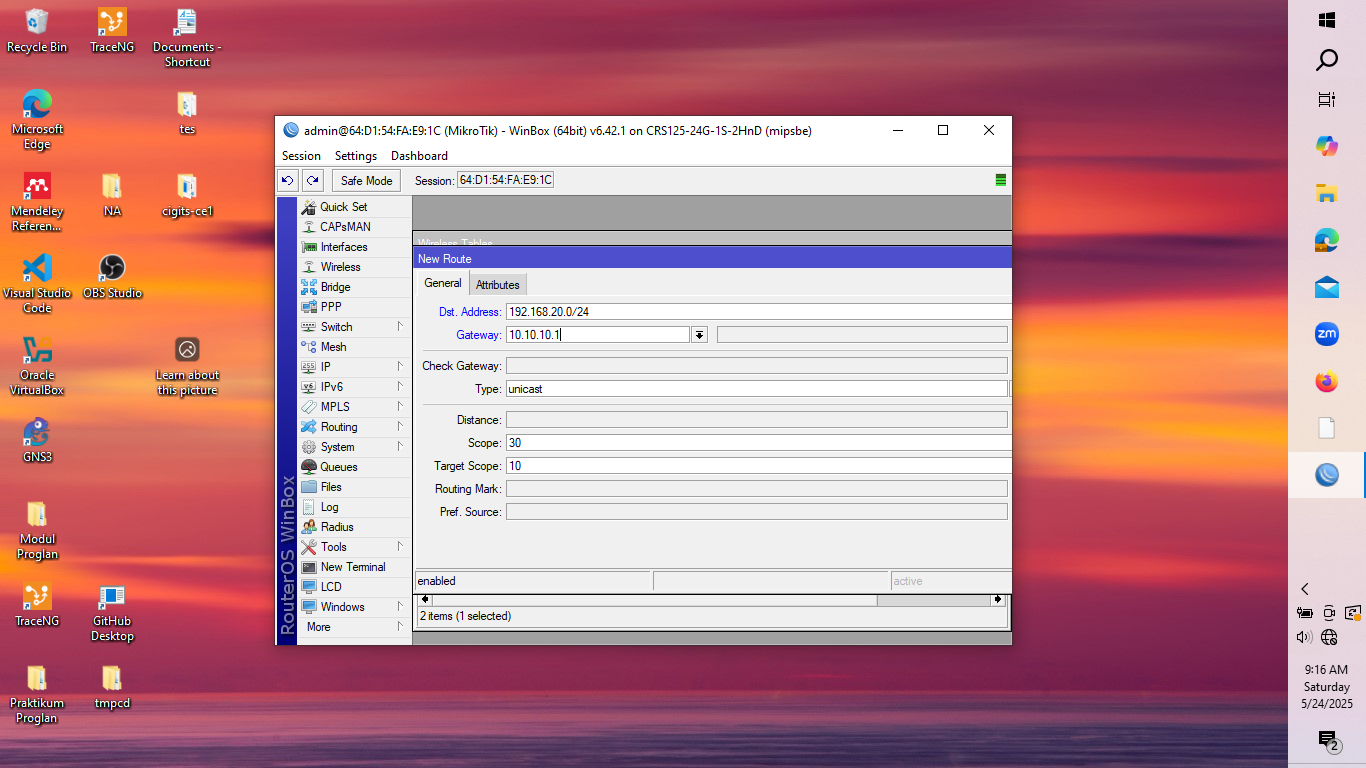
\includegraphics[width=0.5\linewidth]{gambar5.png}
        \caption{Routing Statis pada Router A dan B (Bridge)}
        \label{fig:routing-bridge}
    \end{figure}

    
    \begin{figure}[H]
        \centering
        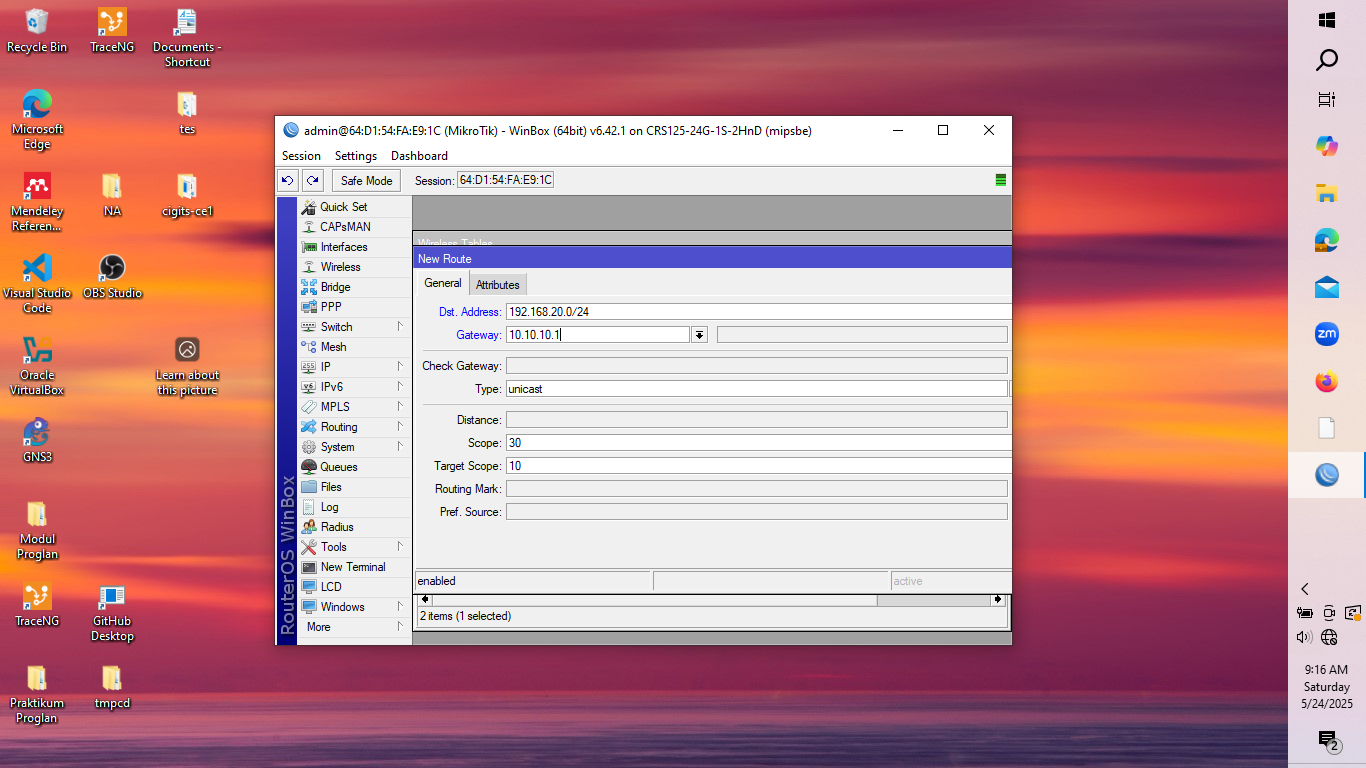
\includegraphics[width=0.5\linewidth]{gambar5.png}
        \caption{Konfigurasi IP Address Laptop (Bridge)}
        \label{fig:ip-laptop-bridge}
    \end{figure}
    
    
    \begin{figure}[H]
        \centering
        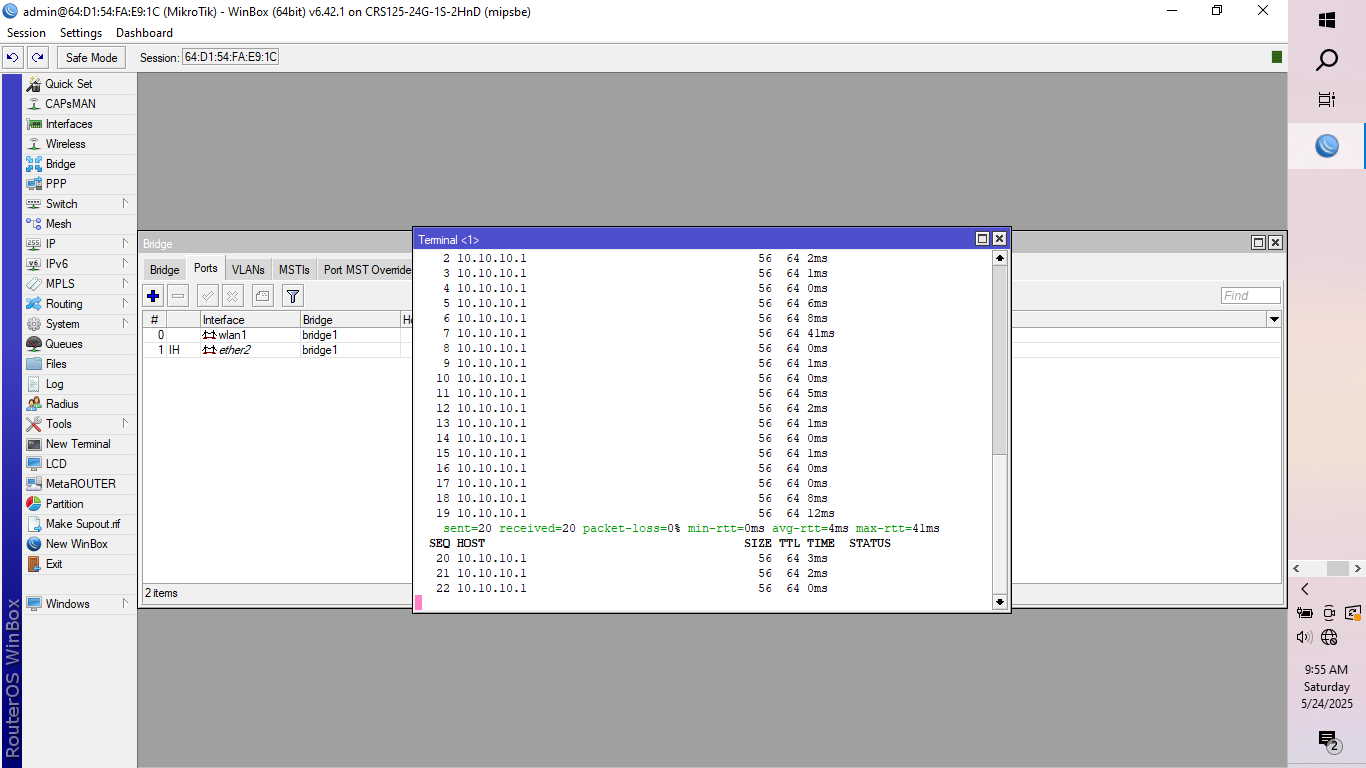
\includegraphics[width=0.5\linewidth]{ping3.png}
        \caption{Ping antara Laptop A dan B (Bridge)}
        \label{fig:ping-bridge}
    \end{figure}

